\documentclass[conference]{IEEEtran}

\usepackage{amsmath,amssymb,mathtools}
\usepackage{graphicx}
\usepackage{booktabs,tabularx,array}
\usepackage{algorithm}
\usepackage{algorithmic}
\usepackage{cite}
\usepackage{url}

\title{Hierarchical Hybrid Planning for Multi-AGV Scheduling in Multi-Floor Factories}

\author{\IEEEauthorblockN{Author Name(s)}
\IEEEauthorblockA{Department or Organization\\
City, Country\\
email address}}

\begin{document}
\maketitle

\begin{abstract}
Multi-floor manufacturing requires automated guided vehicles (AGVs) to share
both floor routes and lift resources. We reimplement the prioritized
multi-AGV scheduling baseline of Guo et al. and evaluate a hierarchical
extension in which a central planner assigns jobs and books lifts while
floor-level planners schedule local route legs using lift lobbies as waiting
points. In the tested three-floor layout, the hybrid configuration reduces
mean makespan by 65\%, total tardiness by 72\%, and load imbalance by 80\%
relative to the paper-style centralized configuration over ten job sets of
100 jobs and 20 AGVs. A centralized FCFS-leg ablation produces the same
schedules as the hybrid on the tested seeds, so the measured schedule gains
are associated with lobby waiting and FCFS leg ordering; floor decomposition
changes where reservation state and computation are held. Five-floor
sensitivity and finite-lobby experiments show that outcomes depend on layout
and capacity-handling choices, with some centralized finite-capacity runs
failing verification. All reported successful plans pass an independent
checker. These simulation results apply to the tested layouts, seeds, and
parameters; they do not establish a general scalability or optimality claim.
\end{abstract}

\begin{IEEEkeywords}
Automated guided vehicles, multi-agent path finding, prioritized planning,
multi-floor logistics, lift coordination, hierarchical scheduling.
\end{IEEEkeywords}

\section{Introduction}

Automated guided vehicles (AGVs) are a central part of material handling in
smart manufacturing. They move workpieces between storage, processing, and
delivery locations, allowing production systems to respond flexibly to
changing orders and workloads. As factories grow, however, coordinating a
fleet becomes a joint assignment, routing, and traffic-management problem.
Vehicles may need the same narrow aisle, workstation approach, or transport
resource at overlapping times. A schedule must therefore assign jobs and
produce routes and timings that avoid collisions while meeting operational
targets such as completion time, delivery due dates, and balanced vehicle
utilization. These requirements become more demanding in multi-floor
facilities, where lifts connect otherwise separate floor networks. A lift is
a shared resource with finite capacity and non-negligible travel time: a
conflict at one lift can delay routes on several floors and propagate through
the entire schedule.

Many AGV scheduling methods centralize assignment and traffic planning. This
provides a system-wide view, but it also concentrates computation and
reservation state at one server. As the fleet and route set grow, that server
must reason about an increasing number of node and track occupancy windows,
including interactions among vehicles operating in different areas. The
planning workload and shared state can consequently become a bottleneck.
This challenge is especially relevant to multi-floor factories: a central
planner must coordinate local floor traffic as well as cross-floor lift
movements. A practical architecture should retain enough central coordination
to prevent conflicting lift use while distributing the detailed routing and
traffic state across the factory.

Guo et al. present a prioritized planning method for large-scale multiple-AGV
scheduling in smart manufacturing \cite{guo2024}. Their approach assigns
transport tasks and plans AGV routes sequentially according to priority,
resolving conflicts with respect to plans already made for higher-priority
vehicles. This provides the centralized baseline for the present work. In
that baseline, assignment and conflict-free routing are handled by a single
planning process \cite{guo2024}.

This paper extends that prioritized-planning baseline with a hybrid
central-plus-edge architecture for a multi-floor factory. A central server
performs job assignment and divides each AGV route into floor-level legs. It
also books the lift trips, which remain shared across floors and therefore
require system-wide coordination. Each floor has an edge server that plans
its local route legs and resolves node and track conflicts using the
prioritized conflict-free routing procedure. The decomposition limits each
floor server's detailed reservation state to its own floor, while the central
server retains responsibility for assignments and inter-floor transitions.
To give vehicles a safe place to wait near a local conflict or a busy lift,
the layout adds a lobby node at each lift landing. A floor server can delay a
leg at its entry lobby, and the central server can schedule a lift departure
after the lift resource becomes available. These lobbies provide waiting
points near the conflict rather than requiring every delay to be absorbed at
the factory's single parking node.

The implementation is evaluated against two centralized configurations: the
paper-style planner, and a centralized planner with the same lift lobbies as
the hybrid system. The saved comparison uses 100 jobs and 20 AGVs over 10
random seeds; each generated plan is checked by an independent verifier. In
the reported mean results, the hybrid configuration reduces last-delivery
makespan by 65\%, total tardiness by 72\%, and usage-time imbalance by 80\%
relative to the paper-style centralized configuration. Its busiest-server
planning CPU time is also lower. These figures describe the project's
modeled factory, parameters, and tested seeds; they should be read as
experimental results for this setup, not as general guarantees for all
multi-floor factories. The comparison also includes a fleet-size sweep over
4, 8, 12, 16, and 20 AGVs, providing a view of how the measured scheduling
metrics vary with fleet size \cite{projectRepo}.

The remainder of the paper is organized as follows. Section~\ref{sec:related}
reviews related work; Section~\ref{sec:model} defines the scheduling model;
Section~\ref{sec:methods} describes the prioritized and hybrid methods;
Section~\ref{sec:experimental-setup} gives the experimental setup;
Sections~\ref{sec:results-discussion} and~\ref{sec:priority-wait-fairness}
report performance and fairness results; Section~\ref{sec:limitations}
discusses the scope and limitations; and Section~\ref{sec:conclusion}
concludes the paper.

\subsection*{Contributions}
\begin{itemize}
  \item Reimplementation of the ICARCV 2024 prioritized-planning baseline,
        including fixes to the original demo's documented bugs.
  \item A hybrid architecture that separates central job assignment and lift
        booking from per-floor conflict-free route planning.
  \item Lift-lobby waiting points that allow delays to be absorbed near
        floor-level conflicts and lift resources.
  \item Independent verification of completed plans for node and track
        conflicts, edge travel times, dwell windows, route endpoints, and
        exactly-once job assignment.
  \item Comparative results over ten random seeds and a fleet-size sweep.
\end{itemize}



\section{Related Work}
\label{sec:related}

\subsection{Centralized prioritized planning and conflict search}

Guo et al.'s ICARCV 2024 method is the baseline for this study. It formulates
large-scale multiple-AGV scheduling as prioritized assignment and route
planning, resolving conflicts against previously planned higher-priority
vehicles \cite{guo2024}. The sequential approach avoids joint search over all
vehicle paths, but its result depends on assignment and priority order.
Prioritized wait adjustment instead starts from individual paths and shifts
waiting using safe intervals; its preliminary evaluation reports 50--250
agents and trades solution quality for runtime \cite{andreychuk2018}.

Conflict-based search (CBS) offers a coupled alternative. Continuous-time CBS
methods model nonuniform action durations and geometric collisions
\cite{andreychuk2022}. He et al. extend CBS to multi-floor MAPF with
single-agent elevator occupancy and elevator reset intervals, explicitly
including lift conflicts in search \cite{he2026}. These methods provide
stronger conflict reasoning, while our experiments focus on job assignment,
prioritized route windows, and lift arbitration in a decomposed planner.

\subsection{Distributed multi-robot and AGV coordination}

Distributed manufacturing schedulers assign decisions to resource agents.
Zhou et al. use collaborative reinforcement-learning schedulers for
heterogeneous smart-factory units and consider rush orders and machine
failures \cite{zhou2021}. Maoudj et al. formulate a capacitated multi-AGV
scheduling problem with conflicting products and compare a decentralized
multi-agent approach with a mixed-integer model \cite{maoudj2023}. Draganjac
et al. present decentralized traffic management based on local coordination
for free-ranging industrial vehicles \cite{draganjac2020}. These works
address decentralized decisions or online manufacturing dynamics; they do
not evaluate the same combination of a central lift calendar and floor-local
route-leg reservations used here.

\subsection{Hierarchical and zone-based planning}

Spatial decomposition reduces the planning scope by assigning agents to
regions or layers. The spare-zone method of Zhao et al. uses a hierarchical
allocation layer and local coordination to resolve collisions and deadlocks
for vehicles following fixed paths \cite{zhao2021}. Pratissoli et al. use a
centralized, decoupled, multilayer traffic manager with topological sectors,
traffic-aware route planning, and time-expanded coordination in an industrial
setting \cite{pratissoli2024}. HMAPP combines high-level region sequences
with regional conflict-based searches \cite{hmapp2021}; hierarchical
large-scale multirobot replanning similarly combines global congestion-aware
routing and parallel low-level planning \cite{pan2024}. Verma et al.'s
dynamic resource reservation method allows multiple reservations at shared
resource points and can be implemented centrally or with local controllers
\cite{verma2024}. These approaches motivate layered coordination and local
waiting or conflict-resolution areas. The present implementation instead
partitions local route windows by floor while retaining central job
assignment and lift booking.

\subsection{Learning-based and optimization-based AGV scheduling}

Scheduling quality and traffic efficiency have also been addressed with
optimization, learning, and large-neighborhood methods. Wang et al. use a
neural network to predict travel time in a multi-state AGV scheduling method
for flexible manufacturing \cite{wang2022}. Lu et al. combine workstation
assignment rules with a space-time scheduling model and cooperative
optimization for conflict-free AGV routes \cite{lu2023}. Hu et al. combine
reservation timetables, task allocation, and variable-neighborhood search
for multi-load AGVs; their experiments include fleets from 3 to 200 vehicles
\cite{hu2022}. MAPF-LNS2 repairs collisions by repeatedly replanning subsets
of agents and reports results up to 8,000 agents on a congested warehouse
benchmark under a one-hour limit \cite{mapflns2022}. These approaches target
search quality, assignment, or scale, but the cited formulations do not
evaluate our specific central-lift and floor-server split.

\subsection{Multi-floor warehouses and lifts}

Elevator-aware warehouse routing is studied directly by Ma et al. for a
double-warehouse system connected by elevators \cite{ma2014}. Werner analyzes
MAPF in high-rack warehouses where agents remain on their assigned levels
and elevators transport goods vertically; the method constructs waiting
zones for elevator use \cite{werner2025}. He et al.'s CBS-E formulation
models elevator capacity and reset-time conflicts \cite{he2026}. These
papers demonstrate that lift state and waiting near elevator shafts matter
to multi-floor routing. Our evaluated contribution combines this resource
with prioritized job assignment, floor-local route-leg planning, and
central lift booking. The claim is limited to this implemented combination
and the experiments in this paper; we make no claim of priority over all
related systems.

\subsection{Contributions}

This work reimplements the ICARCV 2024 prioritized-planning baseline with
corrections to the original demonstration, then evaluates a hierarchical
central-plus-floor-server extension. The central component assigns jobs and
books lifts, floor planners resolve local route conflicts, and lift-lobby
waiting points support delays near floor transitions. An independent checker
validates completed schedules. Results compare centralized, FCFS, and hybrid
variants over seeded job sets, fleet sizes, job scales, and parameter settings
for the tested factory layouts \cite{projectRepo}.

\section{Problem Model}
\label{sec:model}
The model uses the prioritized assignment and route-window notation of the
ICARCV baseline \cite{guo2024}, with explicit lift and lobby elements for a
multi-floor factory.

\subsection{Sets and graph}

Let $G=(N,E)$ be the undirected factory graph. Each undirected edge represents a
bidirectional track. Let $F$ be the set of floors, and let $N_f\subseteq N$
denote the nodes on floor $f\in F$. Let $L\subseteq E$ be the set of lift links
between floors. The parking node is $\pi\in N$.

Let $J$ be the set of jobs and $V$ the set of AGVs. Each job $j\in J$ is served
by exactly one AGV. Let $M_i$ index the successive node visits on AGV $i$'s
route, including repeated visits to the same physical node.

\subsection{Parameters}

For every job $j\in J$, its pickup and delivery nodes are
\[
  p_j\in N,\qquad p'_j\in N,\qquad p_j\ne p'_j,
\]
and $t_j,t'_j$ are its desired pickup and delivery times. The service-time
parameters are $\eta$ (loading) and $\eta'$ (unloading). The safety separation
is $\delta>0$, and AGV speed is $v>0$. Each edge $e\in E$ has length $\ell_e$;
for lift edges $e\in L$, $\ell_e$ is the configured lift length. Travel time
along an edge is
\[
  \tau_{uv}=\frac{\ell_{\{u,v\}}}{v},\qquad \{u,v\}\in E.
\]
Let $d(u,w)$ be the shortest-path travel time between nodes $u,w$, computed
from these edge times. The code uses a fixed weight $\lambda\ge 0$ in its
assignment fitness and a maximum of $k_{\max}$ passes in Algorithm 3.

Jobs are considered in the release order
\[
  j_1,\ldots,j_{|J|}
  =\operatorname{sort}_{j\in J}(t_j,j),
\]
that is, increasing desired pickup time, with job identifier as the tie-breaker.
AGV $i$ has a fixed priority rank $\rho_i$, where smaller values mean higher
priority.

\subsection{Decision and schedule variables}

The assignment variable is
\[
  x_{ji}\in\{0,1\},
\]
where $x_{ji}=1$ means AGV $i$ is assigned job $j$. Each job is assigned once:
\[
  \sum_{i\in V}x_{ji}=1\qquad \forall j\in J.
\]

For each AGV $i$, let
\[
  R_i=(n_{i,0},n_{i,1},\ldots,n_{i,q_i})
\]
be its ordered route, with $n_{i,0}=n_{i,q_i}=\pi$. The implemented planner
constructs $R_i$ by concatenating shortest paths from the AGV's current node
to each assigned job's pickup and delivery nodes, then back to $\pi$.

For visit $m\in M_i$, let $lt_{im}$ and $rt_{im}$ be the start and end of its
node-occupancy window. Its dwell time is $dwell_{im}$, equal to $\eta$ at a
pickup, $\eta'$ at a delivery, and zero at a pass-through visit. The edge
occupancy window for consecutive visits $m-1,m$ is
\[
  [rt_{i,m-1},lt_{im}],
\]
with duration fixed to the edge travel time:
\[
  lt_{im}-rt_{i,m-1}=\tau_{n_{i,m-1},n_{i,m}}.
\]
Thus, the AGV does not stop while traversing an edge. At ordinary nodes,
\[
  rt_{im}-lt_{im}=dwell_{im}.
\]
The parking node is exempt from node-conflict checks and may have an extended
window to represent waiting.

\subsection{Algorithm 1 assignment quantities}

When job $j$ is considered, let $s_i$ and $vt_i$ be AGV $i$'s current node and
available time. The code computes
\begin{align*}
  ct_{ji}
  &=vt_i+d(s_i,p_j)+\eta+d(p_j,p'_j)+\eta',\\
  et_{ji}
  &=\max\!\left(0,\ t_j-\bigl(vt_i+d(s_i,p_j)+\eta\bigr)\right),\\
  dt_{ji}
  &=\max(0,\ ct_{ji}-t'_j),\\
  F_{ji}
  &=ct_{ji}+\lambda(et_{ji}+dt_{ji}).
\end{align*}
The job is assigned to the AGV minimizing $F_{ji}$; ties are broken by AGV
priority. After assignment, $vt_i$ and $s_i$ are updated to $ct_{ji}$ and
$p'_j$, respectively.

\subsection{Conflict separation and start delays}

Let $W_n$ be the fixed occupancy windows of higher-priority AGVs at ordinary
node $n$. Let $W'_{uv}$ be the fixed edge windows on directed traversal
$u\to v$. In the implementation, a physical track is exclusive in both
directions: edge conflicts are checked against windows for both $u\to v$ and
$v\to u$.

For two different AGVs $i\ne h$, overlapping use of an ordinary node or the
same bidirectional track must be separated by at least $\delta$. For occupancy
intervals $[a,b]$ and $[c,d]$, the required separation is
\[
  c\ge b+\delta
  \quad\text{or}\quad
  a\ge d+\delta.
\]
The parking node $\pi$ is exempt from node separation. Algorithm 3 resolves a
conflict by shifting a prefix of the current route to the right. It computes
the cumulative start delay $st^*$ by sweeping backward from the conflict visit
to the nearest previous exempt node, using the window function
$f(lt,rt,W)$. After the sweep, the affected node and edge windows are shifted
by $st^*$, and the previous parking window is extended by the same amount. The
sweep is limited to $k_{\max}$ passes; if exhausted, the implementation applies
its fallback delay.

\subsection{Interpretation and assumptions}

This is the implemented scheduling procedure rather than a single globally
optimized mixed-integer program. It first assigns jobs greedily in pickup-release order
using $F_{ji}$, fixes shortest-path routes, then schedules AGVs in priority
order and resolves conflicts through Algorithm 3. It assumes known job times,
fixed AGV priorities, constant speed, fixed edge travel times, service time
only at pickup and delivery, no stops on edges, and exclusive use of each
bidirectional track. The implemented centralized model allows waiting only at
$\pi$; lift-lobby waiting points are an additional hybrid-layout feature.

\subsection{Hard feasibility constraints}

The following conditions express the hard checks performed by the independent
verifier. Let $P_{im}=[lt_{im},rt_{im}]$ be the window for
visit $m$ of AGV $i$, and let $\mathcal{B}$ be the set of exempt waiting nodes.
For the centralized layout, $\mathcal{B}=\{\pi\}$; in the hybrid layout it
also contains lift lobbies. Write $\varepsilon$ for the verifier's numerical
tolerance.

\paragraph{Route endpoints and initial time.}
Every AGV starts at the parking node at time zero and finishes at that node:
\[
  n_{i,0}=\pi,\qquad n_{i,q_i}=\pi,\qquad |lt_{i,0}|\le\varepsilon
  \qquad (i\in V).
\]

\paragraph{Node conflict avoidance.}
For each ordinary node $n\in N\setminus\mathcal{B}$, distinct AGVs may not
occupy it within the safety separation. For every pair of visits $(i,m)$ and
$(h,r)$ to $n$, where $i\ne h$, the windows must satisfy
\[
  rt_{im}+\delta\le lt_{hr}
  \quad\lor\quad
  rt_{hr}+\delta\le lt_{im}.
\]
No node-conflict constraint is imposed on $n\in\mathcal{B}$: parking and
lobbies are exempt and may hold multiple waiting AGVs.

\paragraph{Track conflict avoidance in both directions.}
For each physical track $e=\{u,v\}\in E$, define the traversal window for a
visit transition $m-1\to m$ by
\[
  Q_{im}=[a_{im},b_{im}]
  =[rt_{i,m-1},lt_{im}],
  \qquad \{n_{i,m-1},n_{i,m}\}=e.
\]
For every pair of traversals of the same physical track by distinct AGVs,
including traversals in opposite directions, require
\[
  b_{im}+\delta\le a_{hr}
  \quad\lor\quad
  b_{hr}+\delta\le a_{im}.
\]
This is the verifier's bidirectional-track rule: use of $u\to v$ conflicts
with both $u\to v$ and $v\to u$ use by another AGV.

\paragraph{No pause on an edge.}
Every edge window has exactly the edge's non-stop travel duration:
\[
  lt_{im}-rt_{i,m-1}
  =\tau_{n_{i,m-1},n_{i,m}}
  =\frac{\ell_{\{n_{i,m-1},n_{i,m}\}}}{v}
  \qquad (m=1,\ldots,q_i).
\]

\paragraph{Dwell times.}
Let $\mathcal{P}_{im}$ and $\mathcal{D}_{im}$ indicate that visit $(i,m)$
performs a pickup or delivery, respectively. With at most one service event
per visit, define
\[
  d_{im}=\eta\,\mathcal{P}_{im}+\eta'\,\mathcal{D}_{im}.
\]
At every non-exempt node, dwell must include the required service time (and is
zero at pass-through visits in the constructed plans):
\[
  rt_{im}-lt_{im}=d_{im}
  \qquad(n_{i,m}\notin\mathcal{B}).
\]
At an exempt parking or lobby visit, the verifier only requires the window to
be at least as long as any service dwell there:
\[
  rt_{im}-lt_{im}\ge d_{im}
  \qquad(n_{i,m}\in\mathcal{B}),
\]
so the excess duration can represent waiting. In the implemented job routes,
$\eta$ is used only at pickup events, $\eta'$ only at delivery events, and
pass-through visits have zero dwell.

\paragraph{Exactly-once job service.}
Let $z_{ij}$ be the number of times job $j$ appears in AGV $i$'s assigned-job
list. Every job must be assigned to exactly one AGV:
\[
  \sum_{i\in V}z_{ij}=1\qquad(j\in J),\qquad z_{ij}\in\mathbb{Z}_{\ge0}.
\]
Equivalently, the multiset union of all AGV job lists must equal the job set,
with each job occurring once. The verifier also requires exactly one pickup
and one delivery event for each job, at the specified stations and on the
assigned AGV, with pickup preceding delivery and pickup completion preceding
delivery completion.

\subsection{Algorithm 3 start-delay conditions}

For a conflict at visit $p$, Algorithm 3 chooses a nonnegative cumulative
right-shift $st^*\ge0$ for the route segment after the nearest preceding
exempt node $q$ through $p$. In the no-fallback case, its update is
\[
  lt'_{im}=lt_{im}+st^*,\qquad rt'_{im}=rt_{im}+st^*
  \quad(q<m\le p),\qquad
  rt'_{iq}=rt_{iq}+st^*.
\]
The last equality extends the waiting window at the exempt node. Edge windows
within the shifted segment move consistently because both endpoint times are
shifted; the connecting edge from $q$ is delayed by extending $rt_{iq}$. The
algorithm accumulates the smallest right-shifts needed to clear the fixed
higher-priority windows encountered in its backward sweep, while checking
that a feasible shift does not cross the next blocking window (the $mt^*$
bound). It repeats up to $k_{\max}$ passes. If those passes are exhausted,
the code uses its fallback shift so the AGV waits at the previous exempt node
until higher-priority traffic is free. The independent verifier subsequently
checks the resulting complete plan.

\subsection{Reported objectives}

The implementation reports three performance measures. Let $C_j$ be the
actual delivery-completion time of job $j$ in the final plan, and let $U_i$
be AGV $i$'s usage time, defined in the code as its return time to $\pi$ when
it serves jobs and zero otherwise. Then
\begin{align*}
  M &= \max_{j\in J} C_j
      &&\text{(makespan, last delivery)},\\
  T &= \sum_{j\in J}\max(0,C_j-t'_j)
      &&\text{(total delivery tardiness)},\\
  I &= \max_{i\in V}U_i-\min_{i\in V}U_i
      &&\text{(load imbalance)}.
\end{align*}
One may state a scalar objective as
\[
  \min\; \alpha M+\beta T+\gamma I,
  \qquad \alpha,\beta,\gamma\ge0,
\]
or a lexicographic objective as
\[
  \operatorname{lexmin}(M,T,I).
\]
These are possible mathematical formulations for comparing schedules; the
code does not choose weights or optimize either combined objective. It uses
$F_{ji}$ greedily for job assignment, then applies prioritized conflict
resolution, and reports $M$, $T$, and $I$ as metrics.

\paragraph{Enforced versus checked conditions.}
Algorithm 2 constructs each route's node and edge windows and calls Algorithm
3 when a new window conflicts with already frozen higher-priority windows.
Algorithm 3 shifts the affected route prefix, extends the preceding exempt
node's window, and thereby enforces conflict avoidance incrementally; in the
hybrid planner, floor servers also plan legs and the central server reserves
lift tracks. The independent verifier does not plan or repair the schedule.
It checks the completed plans for start/end at $\pi$, route continuity,
node and bidirectional-track separation, lift capacity, lobby capacity,
exact edge travel durations, service dwell, and exactly-once pickup and
delivery events at the required stations and in the required order. Thus,
the full-plan conditions are independently checked after Algorithms 2 and 3
construct the schedule.


\section{System Architecture and Methods}
\label{sec:methods}

The method combines the prioritized assignment and route-window procedures of
the centralized baseline \cite{guo2024} with a hierarchical floor decomposition.
The central component assigns jobs, splits routes at lifts, arbitrates lift
use, and merges the resulting schedules. A floor-specific planner constructs
conflict-free timings for its local route legs.

\subsection{Architecture classification}

The architecture is hierarchical and decomposed, with floor-local planning
components; it is not fully decentralized. Job assignment, lift booking,
route-leg dispatch, final-plan merging, and verification remain centrally
orchestrated. Floor planners maintain local node and track reservation sets
$W_n$ and $W'_e$, and resolve conflicts on their own route legs. The central
lift calendar coordinates the cross-floor resource.

Figure~\ref{fig:architecture-flow} summarizes the information flow. The
central-to-floor exchanges are internal planner requests and reservation
responses in the evaluated implementation. The AGVs do not negotiate jobs or
lift slots directly.

\begin{figure}[t]
\centering
\fbox{\parbox{0.94\linewidth}{\centering
Jobs and fleet state $\longrightarrow$ Central planner\\
\emph{Algorithm 1 assignment; route split; lift booking; dispatch}\\
$\longleftrightarrow$ Floor planners $f\in F$\\
\emph{Local route-leg planning with $W_n$ and $W'_e$}\\
$\longrightarrow$ Central merge and independent verification\\
$\longrightarrow$ Complete schedules for AGV execution}}
\caption{Central coordination and floor-local route planning.}
\label{fig:architecture-flow}
\end{figure}

\subsection{Algorithm 1: prioritized job assignment}

Jobs are processed in increasing desired pickup time, with job identifier as
the tie-breaker. For each candidate AGV $i$, the planner evaluates
$F_{ji}=ct_{ji}+\lambda(et_{ji}+dt_{ji})$ using predicted completion time,
pickup earliness, and delivery tardiness. It assigns the job to the AGV with
minimum fitness; ties use fixed AGV priority. The selected AGV's route is
extended through shortest paths to pickup and delivery, with loading and
unloading dwell times $\eta$ and $\eta'$, and is ultimately extended back to
parking $\pi$.

\begin{algorithm}[t]
\caption{Prioritized job assignment}
\label{alg:assignment}
\begin{algorithmic}[1]
\REQUIRE Jobs $J$, AGVs $V$, fitness weight $\lambda$, service times $\eta,\eta'$
\ENSURE Assignment $x_{ji}$ and complete routes $R_i$
\FOR{each $j\in J$ in order $(t_j,j)$}
  \FOR{each $i\in V$}
    \STATE Compute $ct_{ji},et_{ji},dt_{ji}$ from AGV state $(s_i,vt_i)$.
    \STATE $F_{ji}\gets ct_{ji}+\lambda(et_{ji}+dt_{ji})$.
  \ENDFOR
  \STATE Choose $i^*\gets\arg\min_i(F_{ji},\rho_i)$; set $x_{ji^*}\gets1$.
  \STATE Append shortest paths $s_{i^*}\to p_j\to p'_j$ with dwell $\eta,\eta'$.
  \STATE Update AGV state to $(p'_j,ct_{ji^*})$.
\ENDFOR
\FOR{each $i\in V$}
  \STATE Append a shortest path from the final assigned station to $\pi$.
\ENDFOR
\end{algorithmic}
\end{algorithm}

\subsection{Algorithm 2: prioritized conflict-free routing}

Algorithm~\ref{alg:routing} processes AGVs in ascending fixed priority,
$V_1\rightarrow V_{|V|}$. For each route, it constructs node occupancy
windows $[lt_m,rt_m]$ and edge traversal windows. If a window conflicts with a
frozen reservation, Algorithm~\ref{alg:sliding} delays the affected route
segment. The resulting node and track windows are then added to the frozen
sets $W_n$ and $W'_e$. In the paper-style configuration, only parking $\pi$
is an exempt waiting node; the lobby configurations also exempt lift-lobby
nodes.

\begin{algorithm}[t]
\caption{Prioritized conflict-free routing}
\label{alg:routing}
\begin{algorithmic}[1]
\REQUIRE Routes $R_i$, dwell times, priority order $V_1,\ldots,V_{|V|}$
\ENSURE Timed plans and frozen reservations $W_n,W'_e$
\STATE Initialize empty node and edge reservation sets $W_n,W'_e$.
\FOR{each AGV $i$ in priority order}
  \STATE Construct node and edge windows along $R_i$.
  \FOR{each candidate window conflicting with $W_n$ or $W'_e$}
    \STATE Apply Algorithm~\ref{alg:sliding} to delay the route segment.
  \ENDFOR
  \STATE Freeze ordinary node windows in $W_n$ and track windows in $W'_e$.
\ENDFOR
\end{algorithmic}
\end{algorithm}

\subsection{Algorithm 3: sliding-window conflict elimination}

For a candidate interval $[lt,rt]$ and fixed windows $W$, the interval
function $f(lt,rt,W)$ returns the smallest right shift $st$ that clears the
candidate with safety separation $\delta$, together with the available
shift bound $mt$ before the next blocking window. For a conflict at route
visit $p$, the algorithm sweeps backward to the nearest preceding exempt
node $q$, accumulating the route-segment shift $st^*$ and maintaining the
bound $mt^*$. It repeats the sweep up to $k_{\max}$ passes. On exhaustion,
the fallback delays departure at the exempt node until the blocking traffic
is free. The shifted windows from $q+1$ through $p$ move by $st^*$, and the
window at $q$ is extended by that delay.

\begin{algorithm}[t]
\caption{Sliding-window conflict elimination}
\label{alg:sliding}
\begin{algorithmic}[1]
\REQUIRE Conflict visit $p$, reservations $W$, route $R$, limit $k_{\max}$
\ENSURE Conflict-free shifted windows and delay $st^*$
\STATE Find the nearest preceding exempt visit $q$.
\FOR{$k=1$ to $k_{\max}$}
  \STATE Set $st^*\gets0$ and $mt^*\gets\infty$.
  \FOR{visits $m=p,p-1,\ldots,q+1$}
    \STATE Evaluate $f(lt_m+st^*,rt_m+st^*,W)$; update $mt^*$ and $st^*$.
    \IF{$st^*>mt^*$} \STATE Stop this backward sweep. \ENDIF
  \ENDFOR
  \IF{the sweep completes within $mt^*$} \STATE \textbf{break} \ENDIF
\ENDFOR
\IF{no feasible sweep completed}
  \STATE Apply the fallback delay at $q$ until blocking reservations clear.
\ENDIF
\STATE Shift windows $q+1,\ldots,p$ and extend the window at $q$ by $st^*$.
\end{algorithmic}
\end{algorithm}

\subsection{Hybrid central-plus-floor-server extension}

The hybrid planner cuts each complete route at lift edges into floor-local
legs. Each floor planner schedules a leg using local $W_n$ and $W'_e$; when
needed, the AGV waits at its entry lobby or at $\pi$. The central planner
reserves the lift track at the earliest available time after the AGV is
ready, respecting the safety separation. It then releases the next floor leg
at the arrival lobby and merges floor and lift windows into the complete
plan before verification.

Legs are dispatched using either priority ordering or first-come-first-served
(FCFS). FCFS orders legs by release time, AGV priority, then leg index. The
priority order processes the legs of higher-priority AGVs first and is used
as a decomposition check. In the tested seeds, priority-order hybrid plans
match the centralized-with-lobbies plans. For the principal performance
comparison, configuration C uses FCFS order.

\begin{algorithm}[t]
\caption{Hybrid floor-leg planning and lift booking}
\label{alg:hybrid}
\begin{algorithmic}[1]
\REQUIRE Assigned routes, floor planners, central lift calendar
\ENSURE Merged complete AGV plans
\STATE Split each route into maximal floor-local legs at every lift.
\STATE Insert each initial leg into the dispatch queue using the chosen order.
\WHILE{the queue is nonempty}
  \STATE Remove the next leg and schedule it with its floor planner.
  \IF{the route continues on another floor}
    \STATE Reserve the intervening lift trip centrally.
    \STATE Release the next leg at the arrival lobby after lift travel.
  \ENDIF
\ENDWHILE
\STATE Merge floor-leg and lift windows; independently verify each plan.
\end{algorithmic}
\end{algorithm}

\section{Experimental Setup}
\label{sec:experimental-setup}

The factory graphs, job sets, and planner runs are generated by the project
implementation \cite{projectRepo}.

\subsection{Factory layout}

Experiments use a three-floor factory layout. It contains
three floor graphs with nine operational nodes per floor, for 27 operational
nodes total, connected by 38 edges. Four inter-floor edges represent lifts;
each lift has a configured length of 40~m. The fleet's single parking node is
$\pi=\texttt{1A}$. For configurations with lobbies, an additional lobby node
is inserted at each lift landing. Lobby nodes are waiting locations and are
excluded from the job-station sampling set. Thus, jobs are sampled from the
26 non-parking, non-lobby operational nodes.

\subsection{Jobs and fleet}

The job generator creates each job by sampling two distinct
stations uniformly from the 26 operational nodes: pickup $p_j$ and delivery
$p'_j$. Desired pickup time is drawn uniformly over the 600-second horizon,
\[
  t_j\sim U[0,600].
\]
For each job, an independent slack value is drawn as $s_j\sim U[30,200]$ and
the desired delivery time is set to
\[
  t'_j=t_j+d(p_j,p'_j)+\eta+\eta'+s_j,
\]
where $d(p_j,p'_j)$ is the shortest-path travel time on the factory graph.
The implementation rounds generated times to one decimal place. The random
seed determines the job set; the comparison uses seeds 1 through 10.

The main experiment uses 20 vehicles named \texttt{AGV-01} through
\texttt{AGV-20}, with fixed priority ranks $V_1$ through $V_{20}$ in that
order. The fleet-size sweep repeats the experiment with 4, 8, 12, 16, and 20
AGVs. Unless otherwise specified, the main comparison uses 100 jobs and 20
AGVs per seed.

\subsection{Planning parameters and configurations}

All configurations use loading time $\eta=16$~s, unloading time
$\eta'=16$~s, safety separation $\delta=10$~s, fitness weight $\lambda=1.0$,
and vehicle speed $v=1$~m/s. Lift links use their configured 40~m length, so
their non-stop travel time is 40~s at the specified speed.

The comparison evaluates four configurations on the same generated job sets:
\begin{description}
  \item[A --- Centralized paper.] The centralized prioritized planner with
        waiting permitted at the parking node only; lift landings have no
        exempt waiting lobbies.
  \item[B --- Centralized with lobbies.] The centralized planner uses the
        same route and conflict-planning procedure, with lift-lobby nodes
        added as exempt waiting locations.
  \item[B2 --- Centralized FCFS legs.] A single centralized planner holds all
        reservations and processes route legs in the same FCFS order as C.
  \item[C --- Hybrid.] The hybrid central-plus-floor-server planner uses the
        same lobbies. The central server assigns jobs and books lift trips;
        floor servers plan floor legs in first-come-first-served order
        (\texttt{order="fcfs"}).
\end{description}

The main comparison contains 10 seeds (1--10), 100 jobs, and 20 AGVs for each
of A, B, B2, and C. A separate fleet sweep evaluates 4, 8, 12, 16, and 20
AGVs over the same seeds and job-generation settings. For correctness
checking of the decomposition, the hybrid planner can also be run in priority
order; that check compares its plans with configuration B.

Additional studies use the same job and fleet model unless otherwise noted.
The job-scale sweep fixes 20 AGVs, uses 5 seeds, and tests 50, 100, 200, and
400 jobs for A, B, B2, C, and prioritized wait adjustment. The five-floor
sensitivity study uses 50 jobs, 10 AGVs, 3 seeds, and all combinations of
$\eta\in\{8,16,32\}$~s, $\delta\in\{5,10,20\}$~s, and lift length in
$\{20,40,80\}$~m. The assignment-baseline comparison uses 100 jobs, 20 AGVs,
and 3 seeds; the competing wait-adjustment comparison uses 10 seeds. Lobby
capacity and wait-fairness studies use 100 jobs and 20 AGVs over 10 seeds.

\subsection{Evaluation metrics}

The comparison records the following measures:
\begin{itemize}
  \item \textbf{Makespan:} time at which the last job delivery is completed.
  \item \textbf{Tardiness:} total positive delivery lateness across jobs,
        $\sum_j\max(0,C_j-t'_j)$, where $C_j$ is actual delivery completion.
  \item \textbf{Load imbalance:} maximum minus minimum AGV usage time, where
        usage time is measured until return to parking (zero for an AGV serving
        no jobs).
  \item \textbf{Waiting:} total and maximum per-AGV waiting time at parking
        or lift lobbies.
  \item \textbf{Compute time:} total planning CPU time across servers and CPU
        time at the busiest server; wall-clock planning time is also recorded.
  \item \textbf{Server state:} maximum number of reservation windows held by
        any one server.
  \item \textbf{Communication:} central-to-floor message count and the number
        of window records in the transmitted payload.
  \item \textbf{Conflict-resolution effort:} number of Algorithm~3 calls.
\end{itemize}

The comparison reports means over the ten seeds; the figures also show the
seed range where applicable. Fleet-sweep results report the corresponding
metrics by fleet size.

\subsection{Plan verification}

Every generated schedule is passed to an independent verifier. It evaluates the completed plans
for start and end at $\pi$, node conflict separation (with parking/lobbies
exempt), bidirectional track conflict separation, no pause during edge
traversal, correct node-window dwell duration, and exactly-once job service.
For the main A/B/C comparison, a run is accepted only when the verifier
returns no violations. Configuration C in priority order is additionally
compared against B to check that the server decomposition preserves the
centralized-with-lobbies plans on the tested seeds.

\subsection{Software and execution environment}

The software environment uses Python 3.11 or 3.12 and the dependencies
\texttt{networkx}, \texttt{matplotlib}, \texttt{numpy}, and \texttt{pillow}.
The dependency manifest names these
packages but does not pin their individual versions. The repository does not
record processor, memory, operating-system, or accelerator specifications;
therefore, hardware details and exact installed package versions are not
reported here. Runtime measurements should be interpreted in light of this
missing machine-level metadata.


\section{Results and Discussion}
\label{sec:results-discussion}

Unless stated otherwise, results below are generated by the project
implementation \cite{projectRepo}. The principal comparison uses 100
jobs and 20 AGVs on each of ten job sets (seeds 1--10). A is the centralized
paper-style planner, B is centralized with lobbies, B2 is centralized with
lobbies and FCFS leg order, and C is the hybrid with FCFS leg order. Every
schedule contributing a reported metric in the principal comparison,
job-scale, sensitivity, assignment-baseline, competing-planner, and fairness
experiments passed \texttt{agv\_core.verify()}. The lobby-capacity sweep also
contains B runs that failed verification; those failures and verified-run
counts are reported explicitly below.

\subsection{Correctness and decomposition check}

All A, B, B2, and C plans in the principal comparison pass verification. The
B2 and C schedules match on all ten seeds, and the
priority-order hybrid reproduces B on all ten seeds. In these experiments,
the floor-server split changes reservation state and computation distribution
but not the schedule metrics when the route-leg order is held fixed.

\subsection{Mean performance over ten seeds}

Table~\ref{tab:mean-results} reports the ten-seed means. The percentage
column is C relative to A. In this tested three-floor setup, C reduces
makespan by 65\%, tardiness by
72\%, and imbalance by 80\%. Its busiest-server CPU mean is 8.6~ms versus
99.6~ms for A (91\% lower); total CPU across C's servers is 22.0~ms. B2 and C
have equal scheduling outcomes, so the B2-to-C contrast isolates the floor
server split's measured computation/state distribution rather than a
schedule-quality change.

\begin{table}[htbp]
\centering
\small
\caption{Mean metrics over ten seeds. Percentages compare C with A.}
\label{tab:mean-results}
\begin{tabularx}{\textwidth}{>{\raggedright\arraybackslash}Xrrrrr}
\toprule
Metric & A & B & B2 & C & C vs. A \\
\midrule
Last-delivery makespan (s) & 7,972.4 & 3,705.9 & 2,768.9 & 2,768.9 & $-65\%$ \\
Total tardiness (s) & 316,893.6 & 122,278.8 & 90,104.5 & 90,104.5 & $-72\%$ \\
Load imbalance (s) & 7,149.9 & 2,832.3 & 1,441.2 & 1,441.2 & $-80\%$ \\
Total waiting (s) & 64,689.7 & 27,647.7 & 27,104.5 & 27,104.5 & $-58\%$ \\
Longest AGV wait (s) & 7,133.4 & 2,830.8 & 1,887.7 & 1,887.7 & $-74\%$ \\
Busiest-server CPU (ms) & 99.6 & 17.7 & 19.8 & 8.6 & $-91\%$ \\
Total server CPU (ms) & 99.6 & 17.7 & 19.8 & 22.0 & $-78\%$ \\
Windows on busiest server & 2,030.7 & 1,733.5 & 1,733.5 & 634.5 & $-69\%$ \\
Central--floor messages & 0.0 & 0.0 & 337.2 & 337.2 & --- \\
Algorithm 3 calls & 106.6 & 165.1 & 168.6 & 168.6 & $+58\%$ \\
\bottomrule
\end{tabularx}
\end{table}

Figure~\ref{fig:main-comparison} visualizes the ten-seed means and ranges.
Figure~\ref{fig:gantt-seed7} shows the four plans for the seed-7 job set.

\begin{figure*}[t]
\centering
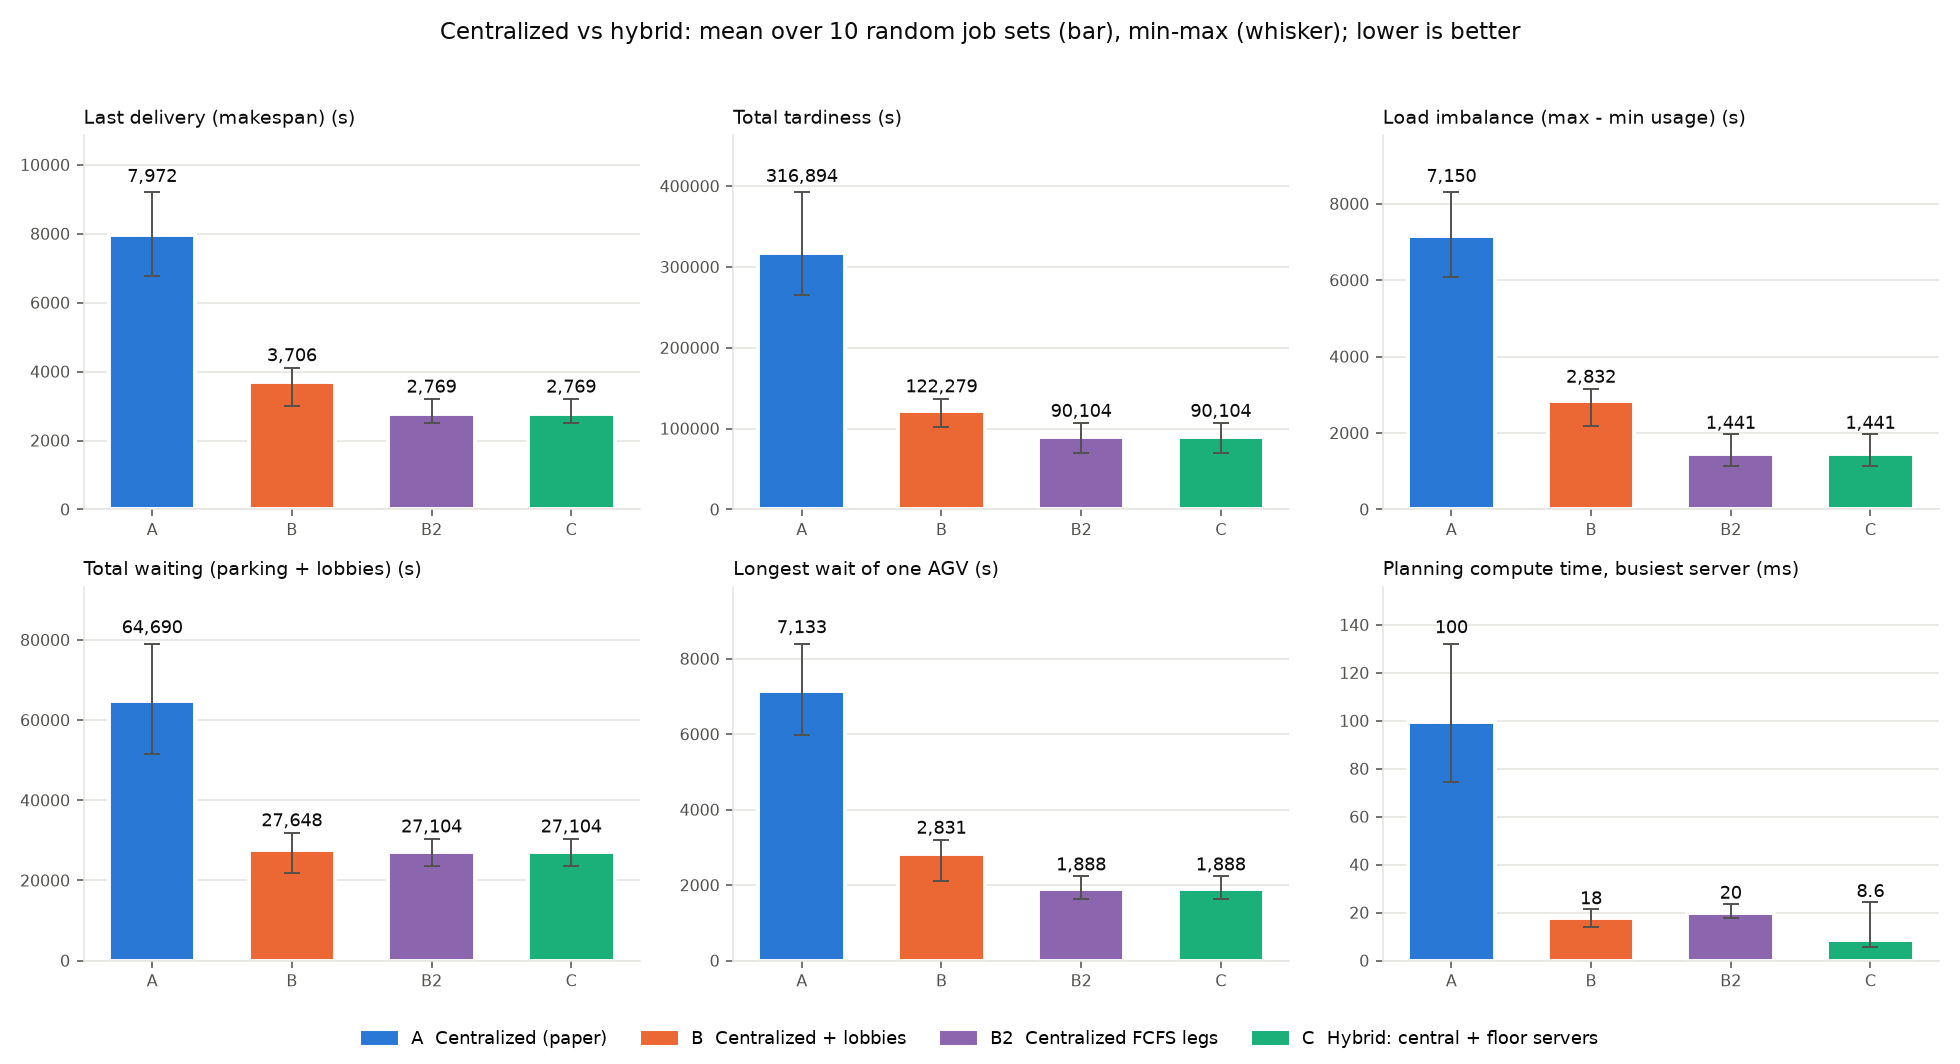
\includegraphics[width=0.98\textwidth]{figures/fig1_compare_metrics.png}
\caption{Mean and min--max range over the ten job sets for A, B, B2, and C.}
\label{fig:main-comparison}
\end{figure*}

\begin{figure*}[t]
\centering
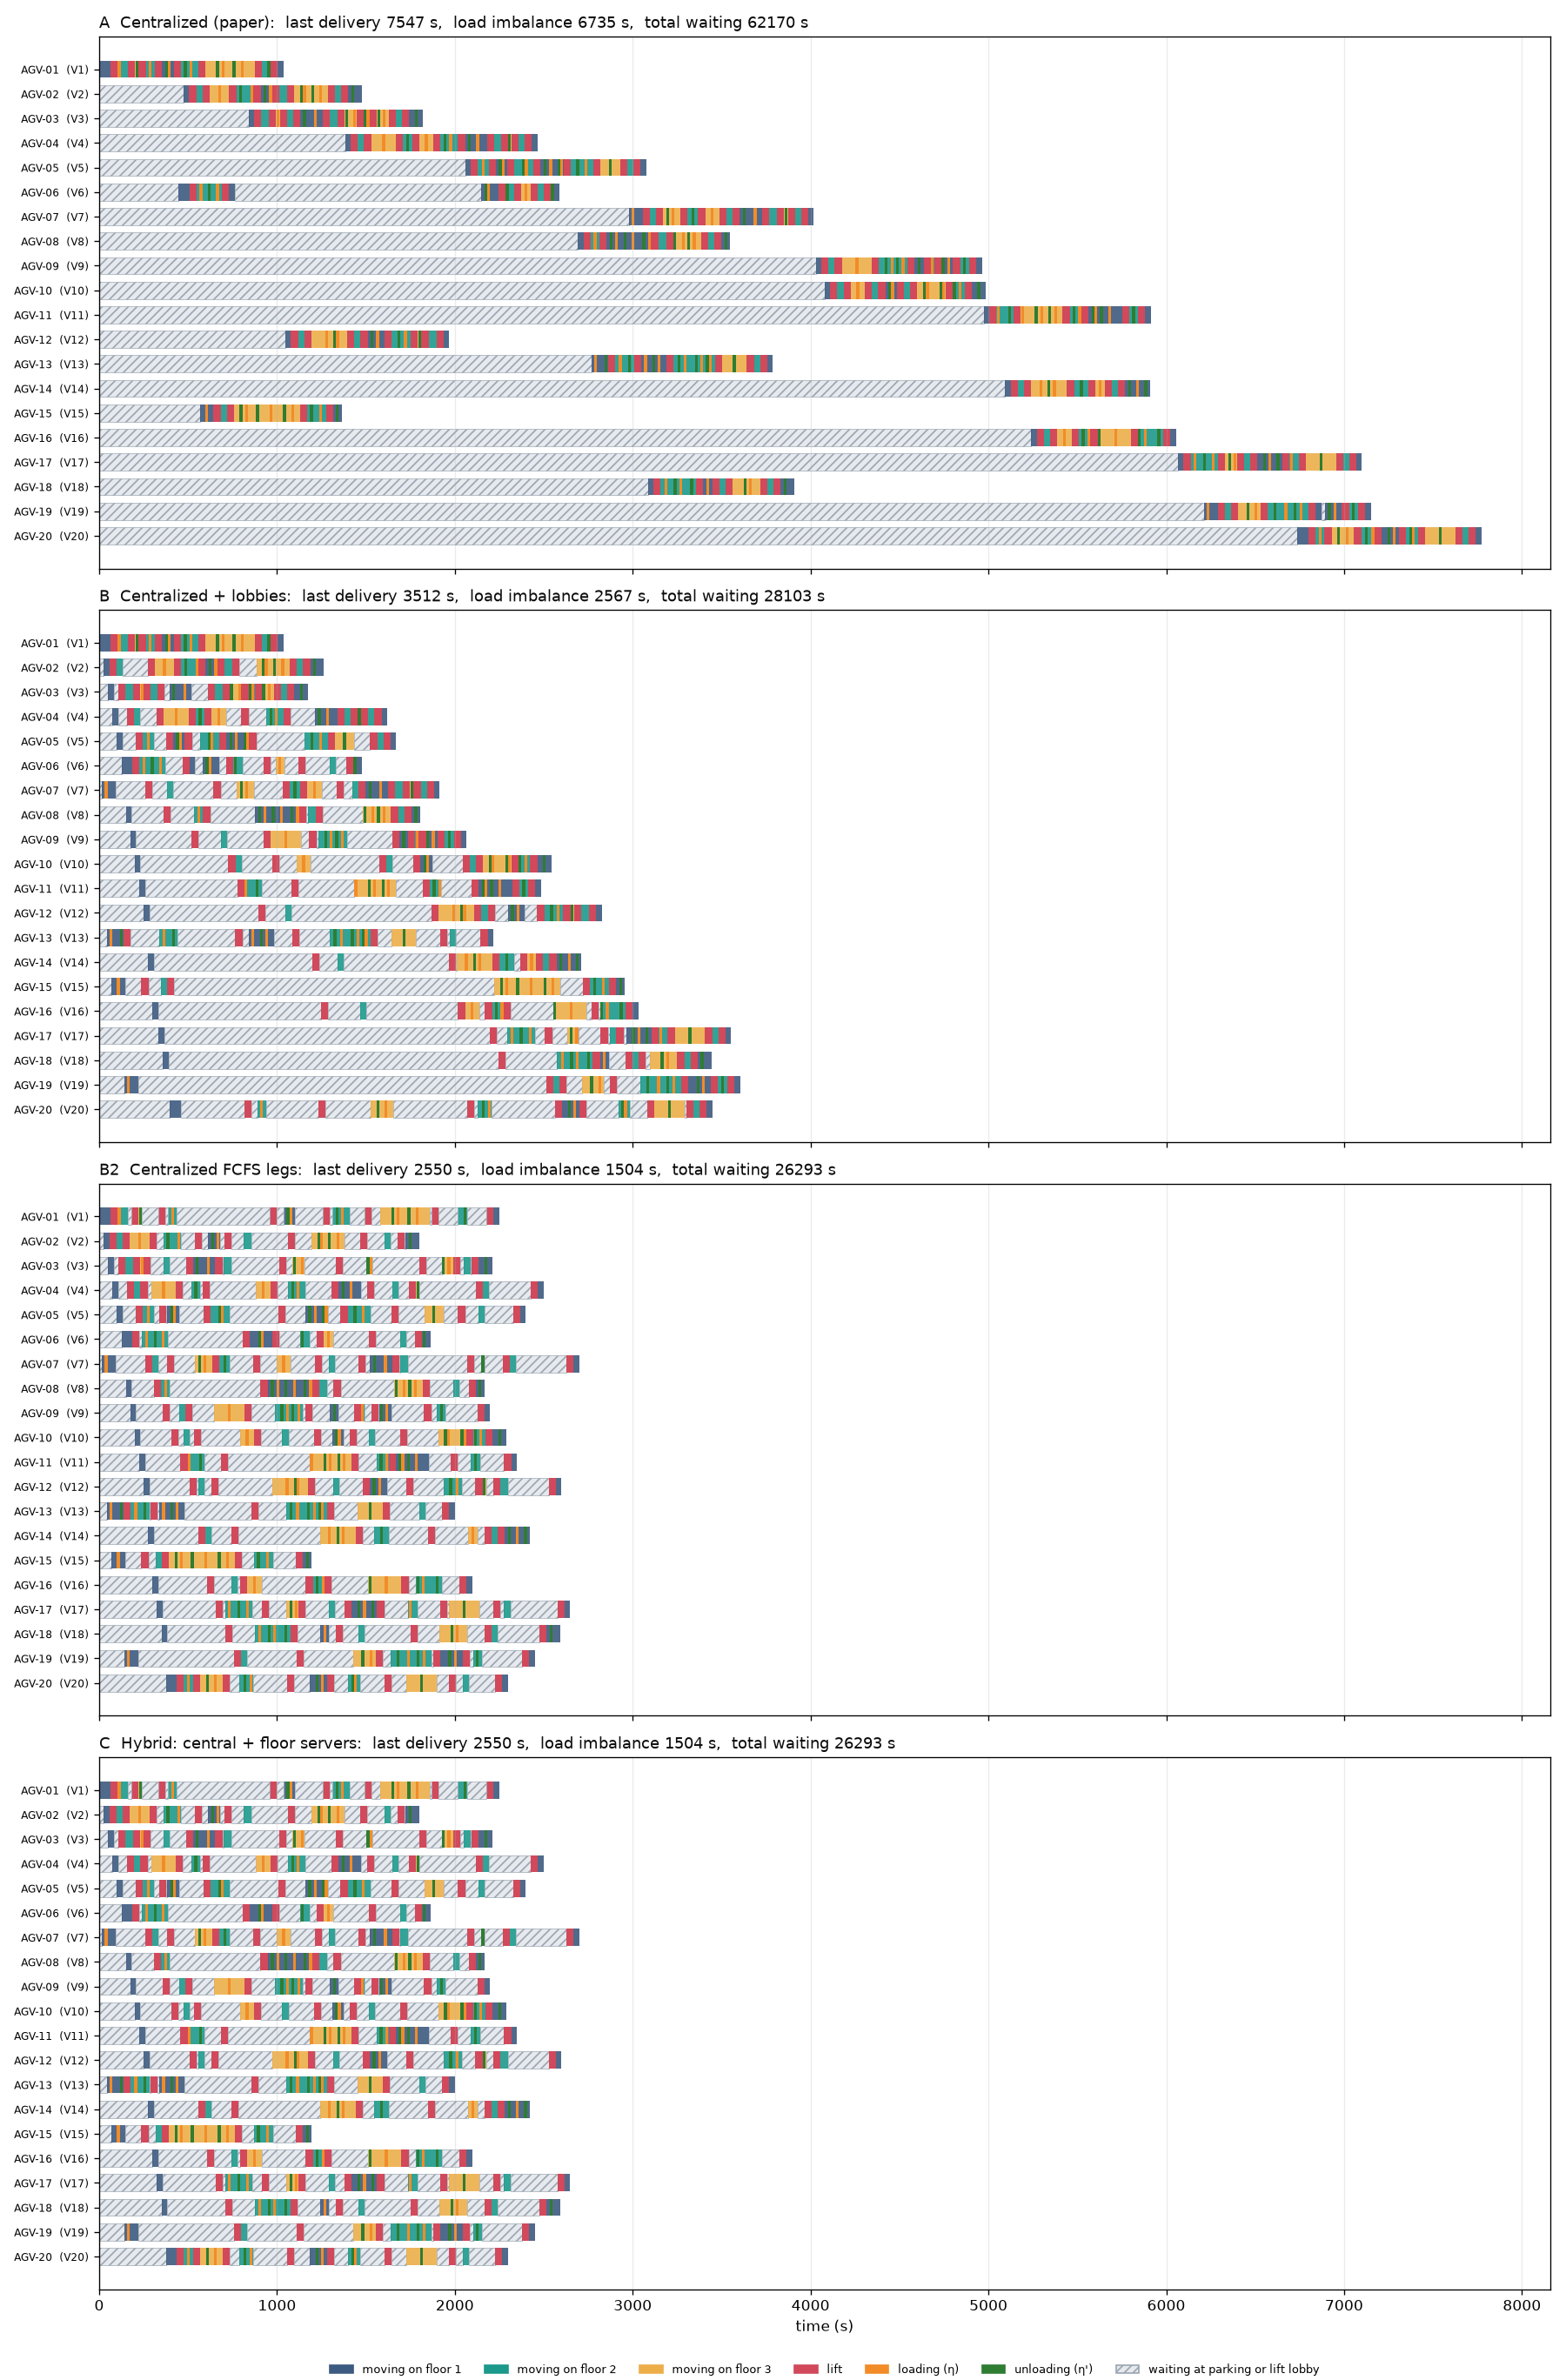
\includegraphics[width=0.9\textwidth]{figures/fig2_gantt_A_B_C.png}
\caption{Schedule timelines for A, B, B2, and C on seed 7. Hatched intervals indicate waiting at parking or lift lobbies.}
\label{fig:gantt-seed7}
\end{figure*}

\subsection{Fleet-size sweep}

Table~\ref{tab:fleet-sweep} gives ten-seed mean imbalance and tardiness.
Tardiness decreases with fleet size for
A at every tested step. For B it decreases through 16 AGVs, then rises from
117,682~s at 16 AGVs to 122,279~s at 20. For B2 and C it decreases slightly
from 90,343~s to 90,104~s over that final step. Thus tardiness does not fall
monotonically in all configurations. Imbalance falls for A and rises for B,
B2, and C over this sweep. B2 and C have the same values at every tested
fleet size.

\begin{table}[htbp]
\centering
\small
\caption{Fleet sweep: mean load imbalance / total tardiness (s), ten seeds.}
\label{tab:fleet-sweep}
\begin{tabular}{rrrrr}
\toprule
AGVs & A & B & B2 & C \\
\midrule
4  & 9,119 / 602,120 & 2,043 / 256,490 & 518 / 235,718 & 518 / 235,718 \\
8  & 8,394 / 453,005 & 2,346 / 149,864 & 788 / 126,223 & 788 / 126,223 \\
12 & 8,249 / 421,464 & 2,456 / 125,292 & 1,145 / 100,319 & 1,145 / 100,319 \\
16 & 7,466 / 348,159 & 2,715 / 117,682 & 1,230 / 90,343 & 1,230 / 90,343 \\
20 & 7,150 / 316,894 & 2,832 / 122,279 & 1,441 / 90,104 & 1,441 / 90,104 \\
\bottomrule
\end{tabular}
\end{table}

Figure~\ref{fig:fleet-sweep} shows all three fleet-sweep metrics.
\begin{figure*}[t]
\centering
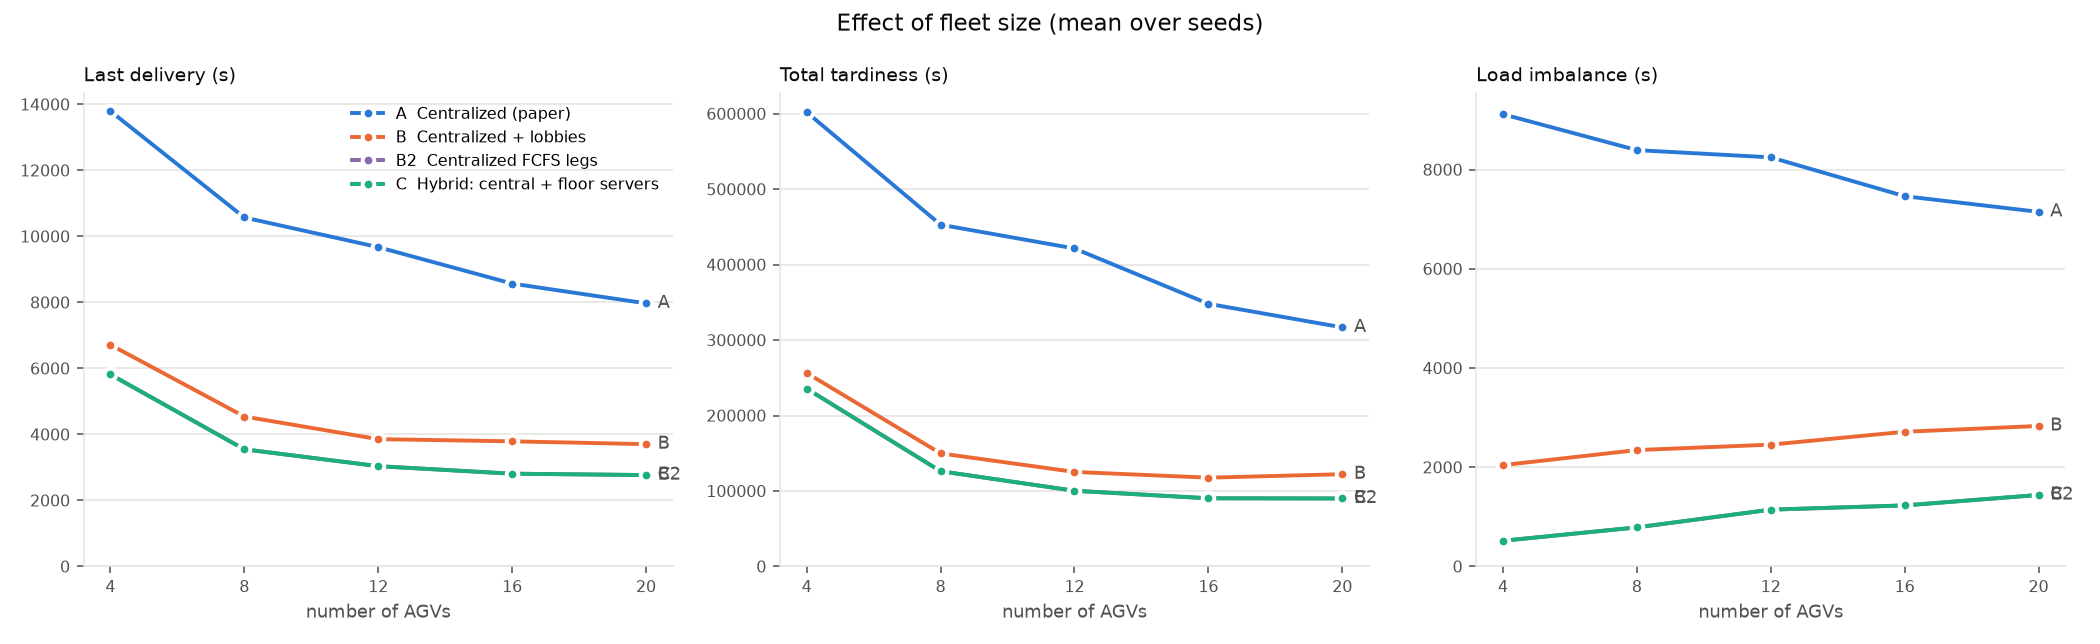
\includegraphics[width=0.98\textwidth]{figures/fig3_fleet_size_sweep.png}
\caption{Mean makespan, tardiness, and load imbalance by fleet size over the tested seeds.}
\label{fig:fleet-sweep}
\end{figure*}

\subsection{Job-scale sweep}

The job-scale experiment fixes 20 AGVs and evaluates 50, 100, 200, and 400
jobs over seeds 1--5. Table~\ref{tab:job-scale} reports C's means and its
percentage reductions relative to A. B2 and C have identical outcomes at each
tested scale. The C-to-A reduction grows across these four tested workload
sizes for all three metrics. This is an observed trend for the tested layout,
fleet, and seeds, not a general scaling guarantee.

\begin{table}[htbp]
\centering
\scriptsize
\caption{Job-scale means: C metrics and C reduction relative to A.}
\label{tab:job-scale}
\begin{tabular}{rrrrrrr}
\toprule
Jobs & C makespan (s) & C tardiness (s) & C imbalance (s) & Makespan reduction & Tardiness reduction & Imbalance reduction \\
\midrule
50  & 1,895.9 & 22,311.8 & 1,425.6 & 58.0\% & 68.3\% & 66.0\% \\
100 & 2,725.3 & 83,285.2 & 1,430.3 & 65.2\% & 72.9\% & 79.6\% \\
200 & 4,674.2 & 360,814.5 & 1,576.1 & 72.6\% & 76.6\% & 89.8\% \\
400 & 8,541.3 & 1,484,910.4 & 2,350.0 & 77.5\% & 78.9\% & 93.3\% \\
\bottomrule
\end{tabular}
\end{table}

\subsection{Parameter sensitivity on five floors}

The sensitivity run covers a five-floor layout, 50 jobs, 10 AGVs, and three
seeds for each of 27 parameter triples: $\eta\in\{8,16,32\}$~s,
$\delta\in\{5,10,20\}$~s, and lift length in $\{20,40,80\}$~m. All 324
configuration rows pass verification. Table~\ref{tab:sensitivity-c} gives
the C means at each level of one factor, averaged over the other two factors
and the three seeds.
The outcomes generally rise with larger $\delta$ and lift length in these
marginal means; the imbalance mean does not rise monotonically with $\eta$.
Because this is a finite grid of settings on one layout, it does not establish
behavior outside that grid.

\begin{table}[htbp]
\centering
\small
\caption{Hybrid C marginal means by parameter value in the five-floor sweep.}
\label{tab:sensitivity-c}
\begin{tabular}{llrrr}
\toprule
Factor & Value & Makespan (s) & Tardiness (s) & Imbalance (s) \\
\midrule
$\eta$ (s) & 8  & 2,377.0 & 36,979.1 & 845.3 \\
$\eta$ (s) & 16 & 2,431.2 & 38,716.9 & 892.2 \\
$\eta$ (s) & 32 & 2,668.6 & 42,874.4 & 811.6 \\
$\delta$ (s) & 5  & 2,290.2 & 34,629.3 & 754.9 \\
$\delta$ (s) & 10 & 2,457.9 & 38,250.9 & 833.5 \\
$\delta$ (s) & 20 & 2,728.8 & 45,690.1 & 960.8 \\
Lift length (m) & 20 & 1,689.3 & 19,697.5 & 557.1 \\
Lift length (m) & 40 & 2,307.7 & 33,839.1 & 797.2 \\
Lift length (m) & 80 & 3,479.9 & 65,033.7 & 1,194.9 \\
\bottomrule
\end{tabular}
\end{table}

\subsection{Assignment baselines}

We regenerated the FCFS and random assignment baselines using the common
Algorithm 2/3 routing planner, for 100 jobs and 20 AGVs over seeds 1--3. All
five configurations passed verification on each seed. Table~\ref{tab:assign}
reports means from the per-seed baseline output.
Under this planner and these three seeds, Algorithm 1's fitness-based
assignment gives little benefit over the FCFS assignment baseline: FCFS has
slightly lower mean makespan, tardiness, and imbalance. Random assignment is
substantially worse on all three measures. This small three-seed comparison
does not establish a general ranking.

\begin{table}[htbp]
\centering
\small
\caption{Assignment baselines: means over seeds 1--3 (100 jobs, 20 AGVs).}
\label{tab:assign}
\begin{tabular}{lrrr}
\toprule
Configuration & Makespan (s) & Tardiness (s) & Imbalance (s) \\
\midrule
A: Algorithm 1 assignment & 7,888.6 & 316,407.8 & 7,048.3 \\
B: centralized with lobbies & 3,687.0 & 120,550.8 & 2,858.9 \\
C: hybrid & 2,783.2 & 84,528.3 & 1,431.9 \\
FCFS assignment & 7,750.5 & 304,553.0 & 6,971.3 \\
Random assignment & 12,322.1 & 493,263.8 & 11,959.8 \\
\bottomrule
\end{tabular}
\end{table}

\subsection{Competing prioritized wait-adjustment planner}

The competing planner (WA) computes individual paths and inserts waits to
avoid conflicts using the same seeded jobs, layout, fleet, speeds, and safety
gap. In the 10-seed, 100-job, 20-AGV comparison, every WA plan passed
verification. Its mean makespan, tardiness, and imbalance were 5,999.9~s,
226,879.9~s, and 5,144.8~s, respectively, compared with 2,768.9~s,
90,104.5~s, and 1,441.2~s for C. The job-scale sweep also reports higher WA
means than C at 50, 100, 200, and 400 jobs. On these tested cases WA did not
outperform the hybrid; this is not evidence that it cannot do so on other
instances.

\subsection{Finite lobby capacity}

The capacity experiment evaluates B and C on three- and five-floor layouts,
100 jobs, 20 AGVs, and ten seeds. Table~\ref{tab:lobby-cap} reports B's
verified-plan counts and means when available, and C's verified counts and
means. The summary describes finite-capacity C as using conservative FCFS
tour admission, with other AGVs waiting at $\pi$ to avoid lobby wait-for
cycles. Its finite-capacity plans verify, but the resulting schedules are
much slower than the unlimited-capacity case. Some B seeds failed plan
verification; that is a planner failure in those runs, not proof that the
underlying scheduling instances are physically infeasible.

\begin{table}[htbp]
\centering
\scriptsize
\caption{Finite-lobby results: verified runs out of ten and mean makespan / tardiness (s).}
\label{tab:lobby-cap}
\begin{tabular}{llrrr}
\toprule
Layout & Capacity $K$ & B verified; mean & C verified; mean \\
\midrule
3 floors & 1 & 0/10; n/a & 10/10; 19,153.1 / 911,565.3 \\
3 floors & 2 & 2/10; 4,108.9 / 146,026.1 & 10/10; 19,153.1 / 911,565.3 \\
3 floors & 4 & 10/10; 3,764.2 / 124,813.4 & 10/10; 19,153.1 / 911,565.3 \\
3 floors & Unlimited & 10/10; 3,705.9 / 122,278.8 & 10/10; 2,768.9 / 90,104.5 \\
5 floors & 1 & 0/10; n/a & 10/10; 26,701.3 / 1,294,641.3 \\
5 floors & 2 & 0/10; n/a & 10/10; 26,701.3 / 1,294,641.3 \\
5 floors & 4 & 9/10; 4,059.7 / 134,817.4 & 10/10; 26,701.3 / 1,294,641.3 \\
5 floors & Unlimited & 10/10; 4,014.8 / 133,751.7 & 10/10; 3,174.2 / 110,421.4 \\
\bottomrule
\end{tabular}
\end{table}

\subsection{Per-server state and computation}

For seed 7, the centralized planner reports 1,989 windows and
109.2~ms CPU on A's central server. C holds 146 windows and uses 6.5~ms on
its central server; its floor servers hold 478, 619, and 454 windows and use
3.2, 6.1, and 5.6~ms, respectively. The largest C server therefore holds
619 windows and uses 6.1~ms in this seed. These seed-specific values are
distinct from the ten-seed means in Table~\ref{tab:mean-results}. The server
state and CPU comparison appears in Figure~\ref{fig:per-server}.

\begin{figure*}[t]
\centering
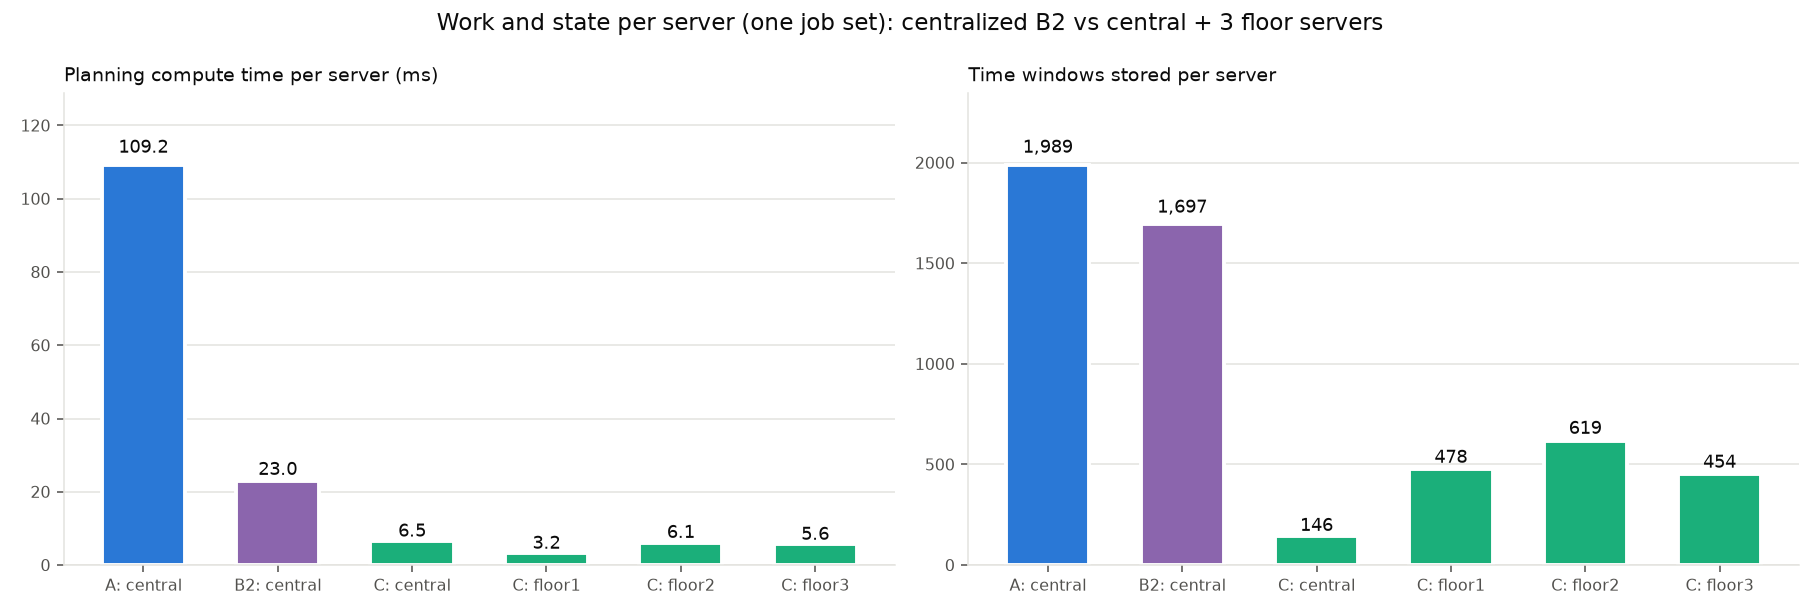
\includegraphics[width=0.98\textwidth]{figures/fig4_per_server.png}
\caption{Per-server computation time and reservation windows for centralized B2 and hybrid C on seed 7.}
\label{fig:per-server}
\end{figure*}

\subsection{Discussion and scope}

In the tested three-floor setting, adding lobbies improves the A-to-B
comparison. Changing B to B2 changes route-leg processing to FCFS and
improves the reported scheduling outcomes. B2 and C then match schedule
metrics, so the additional floor-server split changes measured state and
computation distribution, not schedule quality, in these comparisons. The
five-floor sensitivity and lobby-capacity experiments show that outcomes
depend on parameter values and on the capacity-handling policy. Finite
capacity under the tested conservative admission rule can impose large
delays. The job-scale sweep indicates a larger C-versus-A reduction over the
four tested workloads, while the fleet sweep has the non-monotone B
tardiness result described above. None of these finite experiments establishes
performance outside the layouts, seeds, fleet sizes, and parameters tested.


\section{AGV Waiting-Time Fairness}
\label{sec:priority-wait-fairness}

We measured each vehicle's total wait at parking nodes and lift lobbies for
configurations A, B, B2, and C over seeds 1--10 (100 jobs and 20 AGVs per
seed). Each schedule was checked by the independent verifier; all plans
passed \cite{projectRepo}. The table reports the mean and standard deviation across the
ten per-seed fairness statistics. Pearson and Spearman correlations use the
fixed AGV priority rank (1 is highest); Gini is calculated over per-AGV total
wait. The max/min ratio is infinite whenever any AGV has zero wait.

\begin{table}[htbp]
\centering
\caption{Waiting fairness by configuration, mean $\pm$ standard deviation over ten seeds.}
\label{tab:fairness-configs}
\begin{tabular}{lrrrr}
\toprule
Configuration & Pearson $r$ & Spearman $\rho$ & Gini & Max/min wait \\
\midrule
A   & $0.884\pm0.073$ & $0.886\pm0.074$ & $0.382\pm0.018$ & $\infty$ (10/10) \\
B   & $0.961\pm0.041$ & $0.965\pm0.033$ & $0.354\pm0.016$ & $\infty$ (10/10) \\
B2  & $0.419\pm0.267$ & $0.425\pm0.264$ & $0.143\pm0.036$ & $3.842\pm1.468$ \\
C   & $0.419\pm0.267$ & $0.425\pm0.264$ & $0.143\pm0.036$ & $3.842\pm1.468$ \\
\bottomrule
\end{tabular}
\end{table}

The figure plots mean total wait by fixed priority rank. A and B concentrate
delay strongly toward lower-priority ranks. B2 and C have identical wait
statistics in this experiment, consistent with their identical FCFS leg
ordering and schedules: the floor-server split itself did not change fairness
here. C reduces inequality relative to A and B (lower Gini and a smaller
priority-wait correlation), but the top-ranked AGV waits longer on average in
C (1169.1 s) than under A or B (0 s in each). Thus the hybrid is fairer by
these aggregate distribution and rank-correlation measures, while shifting
some delay onto the highest-priority vehicle; this is not an unqualified
fairness improvement.

\begin{figure}[htbp]
\centering
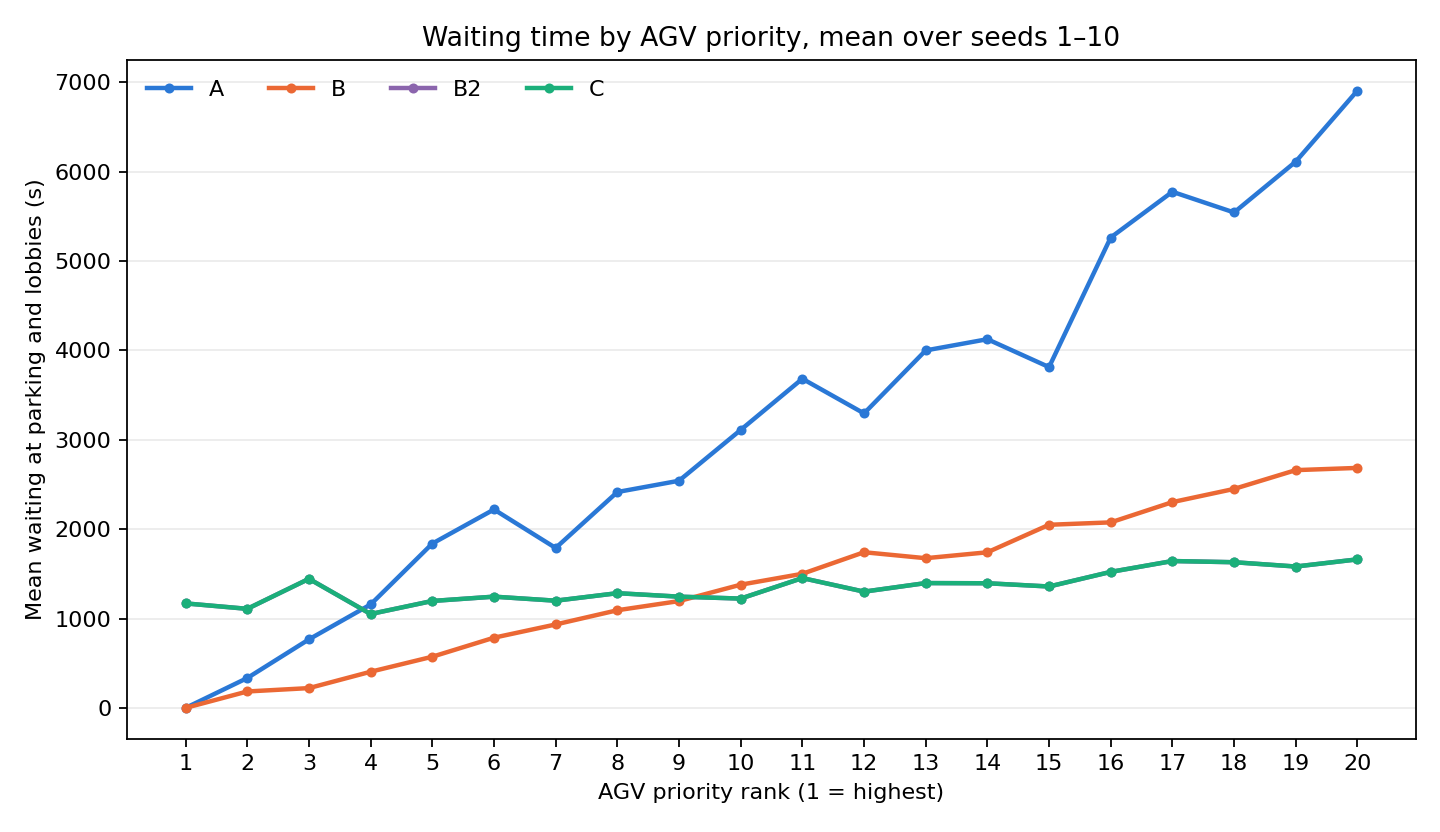
\includegraphics[width=0.9\linewidth]{figures/mean_wait_by_priority.png}
\caption{Mean parking-plus-lobby wait by fixed AGV priority rank over seeds 1--10.}
\label{fig:wait-rank}
\end{figure}

\subsection{Fairness variants on C}

Two simple changes were evaluated on the same ten seeds. In the rotation
variant, job batches rotate the AGV priority ordering. In the waiting-trigger
variant, AGVs whose accumulated wait exceeded 600 s were promoted during
replanning; 600 s is a trigger, not a hard cap. All variant plans passed the
independent verifier.

\begin{table}[htbp]
\centering
\caption{C fairness variants: mean $\pm$ standard deviation over ten seeds.}
\label{tab:fairness-variants}
\begin{tabular}{lrrr}
\toprule
Variant & Makespan (s) & Tardiness (s) & Imbalance (s) \\
\midrule
C (baseline) & $2768.9\pm195.8$ & $90104.5\pm11447.3$ & $1441.2\pm241.1$ \\
C with rotating priority & $2737.6\pm169.7$ & $88009.6\pm10147.2$ & $1425.3\pm250.6$ \\
C with 600 s wait-trigger boost & $2768.9\pm195.8$ & $90104.5\pm11447.3$ & $1441.2\pm241.1$ \\
\bottomrule
\end{tabular}
\end{table}

Rotation lowered the reported mean makespan, tardiness and imbalance slightly,
but the Gini increased from 0.143 to 0.145; it weakened correlation with the
original fixed ranks but did not reduce overall wait inequality. The wait
trigger produced the same schedules and performance metrics as baseline C:
under the current FCFS leg order, priority changes mostly affect ties and did
not alter route-leg order. These results are descriptive for ten seeds; no
significance test was performed \cite{projectRepo}.


\section{Limitations}
\label{sec:limitations}

The results should be interpreted in light of the implementation's scope and
modeling assumptions \cite{projectRepo}. Some are deliberate simplifications that make the
planning procedure testable; others are limitations of the current prototype
that constrain its transfer to operational factories.

First, this is a simulation implementation. It has no robot operating system
(ROS) integration, vehicle localization or control interface, industrial
communications layer, or hardware-in-the-loop evaluation. This is a known
implementation limitation: simulation verification does not establish safe
execution under sensor error, vehicle dynamics, communication delay, or
controller behavior.

Second, each scenario supplies a static set of jobs known before planning.
The planner sorts jobs by desired pickup time and does not handle new arrivals
during execution. This is a deliberate batch-scheduling assumption, but it
limits conclusions about online manufacturing where urgent jobs, cancellations,
or changed deadlines require replanning. The fleet priority order is also
fixed (AGV-01 as $V_1$ through AGV-20 as $V_{20}$); priorities are not updated
to reflect waiting time, task urgency, or changing vehicle state. This
deliberate rule simplifies deterministic comparisons, while potentially
creating unfair delays and making performance dependent on the chosen order.

Third, every generated job is assigned and served exactly once. There is no
job reassignment, task preemption, vehicle breakdown model, or recovery
procedure after a failure. Exactly-once service is part of the modeled
problem, whereas the absence of failure handling is a known limitation for
deployment in factories where vehicles and stations may become unavailable.

Fourth, the parking node $\pi$ is deliberately exempt from node-conflict
checks so multiple AGVs may start and wait there. In the hybrid configuration,
lift lobbies can also be exempt waiting locations; lobby construction is
optional. The model does not impose a finite capacity on these exempt waiting
areas. Real parking bays and lift lobbies may have limited space, so the
assumption can understate congestion and should be revisited for each site.

Fifth, the implementation treats a physical track as exclusive in both
directions: it checks a traversal against reservations for either direction.
This is deliberately stricter than the paper's reverse-edge conflict check
and can reject safe same-direction following schedules. It favors
conservative separation but may overestimate congestion and completion time
relative to facilities that permit controlled following.

Sixth, experiments use one hand-crafted factory graph and one synthetic job
generator. This is a known generalizability limitation: topology, station
placement, task mix, and due-date distributions may differ substantially in
other plants. Finally, travel and lift times are deterministic functions of
edge lengths and speed, with no uncertainty, acceleration, or congestion
variation. The model also omits battery state and charging decisions. These
are deliberate scope choices for isolating route conflicts, but actual
travel-time variation and charging constraints can change feasible routes,
resource contention, and the relative performance of the architectures.


\section{Conclusion}
\label{sec:conclusion}

This paper presented a hybrid architecture for prioritized multi-AGV
scheduling in a multi-floor smart-manufacturing layout. The work began with
an implementation of the prioritized-planning baseline of Guo et al.
(ICARCV 2024) \cite{guo2024}, correcting the original demonstration's documented issues in
conflict resolution, parking-node handling, service-time placement, and
parameterization. The corrected baseline assigns jobs in earliest-pickup
order using a fitness score, constructs shortest-path routes, and schedules
AGVs by fixed priority while eliminating conflicts through sliding-window
delays.

The main architectural contribution divides planning between a central
server and one server per floor. The central server assigns jobs, separates
routes into floor legs, and books shared lift trips. Floor servers construct
conflict-free schedules for their own legs using local node and track
reservations. Lift-lobby waiting points let an AGV wait near the floor-level
conflict or lift that is delaying it. An independent checker validates each
complete plan for route endpoints, node and bidirectional-track conflicts,
edge travel times, dwell windows, and exactly-once job assignment. On the
tested seeds, the hybrid planner in priority order reproduces the centralized
planner with lobbies, providing a check that the route decomposition
preserves that reference schedule under that processing order.

In the saved comparison of 100 jobs and 20 AGVs over ten seeds, the default
FCFS hybrid configuration reduced mean last-delivery makespan by 65\%, total
tardiness by 72\%, and load imbalance by 80\% relative to the paper-style
centralized configuration. The busiest-server CPU time fell by 92\%, and the
maximum number of reservation windows held by one server fell by 69\%. These
results demonstrate the potential value of lobby waiting and floor-level
decomposition for the modeled three-floor factory. They are empirical
results for the tested layout and settings, not a general guarantee of
optimality or of the same improvement at larger scales \cite{projectRepo}.

The reduction in tardiness is substantial, but the mean total tardiness for
the hybrid remains approximately 90,105~s across 100 jobs per seed. This
indicates that conflict resolution and decomposition alone do not ensure
that assigned deliveries meet their desired times. The current job assignment
is greedy and priority-dependent, and delay accumulated by shared routes,
lift use, and safety separation can still move deliveries well past their
targets. Reducing this residual tardiness will require changes to assignment,
sequencing, and resource coordination in addition to distributing the
planning workload.

\paragraph{Future work.}
Future work will extend the static, known-job setting to dynamic job arrivals
and investigate battery limits and charging decisions. The lift model can
be generalized to multiple lifts per floor, with lift capacity and service
policies represented explicitly. A further architectural step is to remove
the central lift-booking server and investigate fully decentralized lift
coordination. Broader comparisons should include auction-based assignment,
deep reinforcement learning (DRL), and conflict-based search (CBS), using
common instances, objectives, and verification rules. The design should also
be validated on physical multi-floor hardware.



\appendices
\section{Reproducibility and Implementation Map}
\label{app:reproducibility}

The experiment outputs and implementation are available in the project
repository \cite{projectRepo}. The following map identifies the source
locations for the algorithms described in the paper; line numbers refer to
the repository version used to prepare this manuscript.

\begin{table*}[t]
\centering
\footnotesize
\caption{Implementation map for the evaluated methods.}
\label{tab:implementation-map}
\begin{tabularx}{\textwidth}{>{\raggedright\arraybackslash}p{0.21\textwidth}>{\raggedright\arraybackslash}p{0.37\textwidth}X}
\toprule
Component & Source location & Relevant implementation \\
\midrule
Assignment and metrics & \texttt{agv\_code/agv\_code/agv\_core.py}, lines 154--211 and 606--649 & Fitness, route construction, Algorithm 1, reported metrics, and centralized pipeline. \\
Conflict scheduling & \texttt{agv\_code/agv\_code/agv\_core.py}, lines 212--231, 268--408 & Interval function, Algorithm 3, route planning, reservation freezing, and Algorithm 2. \\
Independent checking & \texttt{agv\_code/agv\_code/agv\_core.py}, lines 409--567 & Route continuity, service events, node/track/lift/lobby constraints, and verification. \\
Hybrid planning & \texttt{agv\_code/agv\_code/agv\_hybrid.py}, lines 52--157 and 162--297 & Route splitting, floor-leg planning, lift booking, finite-capacity admission, dispatch, and plan merging. \\
Layouts and comparison & \texttt{agv\_code/agv\_code/agv\_layouts.py}, lines 47--90 and 106--137; \texttt{agv\_code/agv\_code/agv\_compare.py}, lines 46--105 and 214--end & Three- and five-floor graphs, configuration runner, seeded comparison, and figures. \\
Additional experiments & \texttt{agv\_code/agv\_code/sweep\_job\_scale.py}; \texttt{sensitivity.py}; \texttt{agv\_baselines.py}; \texttt{agv\_wait\_adjust.py}; \texttt{agv\_fairness\_experiment.py}; \texttt{lobby\_capacity\_sweep.py} & Job scale, parameter grid, assignment baselines, safe-interval planner, fairness variants, and lobby-capacity sweep. \\
\bottomrule
\end{tabularx}
\end{table*}

The regenerated tables use the CSV outputs under the experiment directories:
\texttt{results\_hybrid/comparison.csv} and \texttt{sweep\_agvs.csv};
\texttt{results\_scale/sweep\_jobs.csv};
\texttt{results\_sensitivity/sensitivity.csv};
\texttt{results\_baselines/assignment\_baselines.csv};
\texttt{results\_wait\_adjustment/comparison.csv};
\texttt{results\_lobby\_capacity/capacity\_sweep.csv}; and the per-seed
CSVs in \texttt{results\_fairness/}. Figures included with the paper are
copies of the generated comparison and fairness plots.

From the repository root, install the project dependencies and run the
experiments from the implementation directory:
\begin{verbatim}
cd agv_code/agv_code
pip install -r requirements.txt
python agv_compare.py --seeds 1-10 --jobs 100 --agvs 20
python sweep_job_scale.py
python sensitivity.py
python agv_baselines.py
python agv_compare.py --seeds 1-10 --jobs 100 --agvs 20 --sweep '' --outdir results_wait_adjustment
python lobby_capacity_sweep.py
python agv_fairness_experiment.py
\end{verbatim}

Compile from the \texttt{paper/} directory with a LaTeX installation that
includes IEEEtran and BibTeX:
\begin{verbatim}
pdflatex main.tex
bibtex main
pdflatex main.tex
pdflatex main.tex
\end{verbatim}


\bibliographystyle{IEEEtran}
\bibliography{references}

\end{document}
